% =====================================================================
%  Stargazer for Beamer — demo deck
%  A clean, modern Beamer theme: serif type, blue→black gradient title
%  bars, a top section-navigation strip, a two-tone footer, and a blue
%  rounded title box.  Swap in your own content in this file; the look
%  lives entirely in theme/stargazer-beamer.tex.
% =====================================================================
\documentclass[10pt, aspectratio=169]{beamer}
% =====================================================================
%  "Stargazer" for Beamer — recreates the touying stargazer look:
%  serif type · blue→black gradient title bar · top section-nav strip ·
%  two-tone footer · blue rounded title box.
% =====================================================================
\usepackage{tikz}
\usetikzlibrary{positioning, arrows.meta, calc, shadings}
\usepackage{booktabs}\usepackage{graphicx}
\usepackage{amsmath, amssymb}\usepackage{appendixnumberbeamer}
\usepackage{newunicodechar}
\newunicodechar{⟨}{\ensuremath{\langle}}\newunicodechar{⟩}{\ensuremath{\rangle}}
\newunicodechar{→}{\ensuremath{\rightarrow}}\newunicodechar{⇒}{\ensuremath{\Rightarrow}}
\newunicodechar{—}{---}\newunicodechar{·}{\textperiodcentered}

\usefonttheme{serif}                       % Latin Modern Roman, like stargazer

% ---- palette ----
\definecolor{SgBlue}{HTML}{1763C6}
\definecolor{SgDark}{HTML}{0D0D0D}
\definecolor{AppleBG}{HTML}{FFFFFF}\definecolor{AppleInk}{HTML}{1A1A1A}
\definecolor{AppleBlue}{HTML}{1763C6}\definecolor{AppleGray}{HTML}{6E6E6E}
\definecolor{AppleLine}{HTML}{D9D9D9}\definecolor{AppleSoft}{HTML}{EAF1FB}

\usetheme{default}
\setbeamercolor{normal text}{fg=AppleInk, bg=white}
\setbeamercolor{structure}{fg=SgBlue}
\setbeamercolor{itemize item}{fg=SgBlue}\setbeamercolor{itemize subitem}{fg=AppleGray}
\setbeamercolor{block title}{fg=white, bg=SgBlue}
\setbeamercolor{block body}{fg=AppleInk, bg=AppleSoft}
\setbeamertemplate{navigation symbols}{}
\setbeamertemplate{blocks}[rounded][shadow=false]
\setbeamerfont{frametitle}{series=\bfseries, size=\large}
\setbeamerfont{title}{series=\bfseries, size=\LARGE}

\newlength{\sgm}\setlength{\sgm}{0.8cm}
\setbeamersize{text margin left=\sgm, text margin right=\sgm}

% ---- top strip: horizontal section navigation on black ----
\setbeamercolor{section in head/foot}{fg=white, bg=black}
\setbeamercolor{section in head/foot shaded}{fg=white!45!black, bg=black}
\setbeamerfont{section in head/foot}{size=\scriptsize}
\setbeamertemplate{headline}{%
  \begin{beamercolorbox}[wd=\paperwidth, ht=2.6ex, dp=1.1ex, sep=0pt]{section in head/foot}%
    \hbox to\paperwidth{\hfil\insertsectionnavigationhorizontal{0.92\paperwidth}{}{}\hfil}%
  \end{beamercolorbox}%
}

% ---- gradient title bar (full bleed) ----
\setbeamertemplate{frametitle}{%
  \nointerlineskip
  \hspace*{-\sgm}%
  
\begin{tikzpicture}
    \useasboundingbox (0,0) rectangle (\paperwidth, 0.95cm);
    \shade[left color=SgBlue, right color=SgDark] (0,0) rectangle (\paperwidth, 0.95cm);
    \node[anchor=west, text=white, font=\usebeamerfont{frametitle}] at (\sgm, 0.48cm) {\insertframetitle};
  \end{tikzpicture}%
  \par\vspace{0.45em}%
}

% ---- two-tone footer ----
\setbeamercolor{foot left}{fg=white, bg=black}
\setbeamercolor{foot right}{fg=white, bg=SgBlue}
\setbeamertemplate{footline}{%
  \hbox{%
    \begin{beamercolorbox}[wd=.5\paperwidth, ht=2.8ex, dp=1.3ex, leftskip=\sgm]{foot left}%
      \tiny\insertshortauthor\hfill%
    \end{beamercolorbox}%
    \begin{beamercolorbox}[wd=.5\paperwidth, ht=2.8ex, dp=1.3ex, rightskip=\sgm]{foot right}%
      \hfill\tiny\insertshorttitle\hspace{1.4em}\insertframenumber\,/\,\inserttotalframenumber%
    \end{beamercolorbox}%
  }%
}

% ---- blue rounded title box ----
\setbeamercolor{title box}{fg=white, bg=SgBlue}
\setbeamertemplate{title page}{%
  \vfill
  \begin{beamercolorbox}[wd=\textwidth, sep=16pt, rounded=true, center]{title box}%
    {\usebeamerfont{title}\inserttitle\par}\vspace{0.4em}
    {\usebeamerfont{subtitle}\insertsubtitle\par}
  \end{beamercolorbox}
  \vspace{1.4em}
  {\centering {\color{AppleInk}\insertauthor\par}\vspace{0.3em}{\small\color{AppleGray}\insertinstitute\par}\par}
  \vfill
}

% ---- section pages (full color, optional) ----
\setbeamercolor{section page}{fg=white, bg=SgBlue}
\setbeamertemplate{section page}{%
  \begin{tikzpicture}[remember picture, overlay]
    \fill[SgBlue] (current page.north west) rectangle (current page.south east);
  \end{tikzpicture}%
  \centering\vfill{\usebeamerfont{frametitle}\color{white}\Large\insertsectionhead\par}\vfill}

% =====================================================================
%  Shared macros + TikZ styles used by every theme variant.
%  Expects these colors to already be defined:
%    AppleBG, AppleInk, AppleBlue, AppleGray, AppleLine, AppleSoft
% =====================================================================

\newcommand{\metric}[2]{%
  \begin{minipage}[t]{\linewidth}\centering
    {\fontsize{40}{44}\selectfont\color{AppleBlue}#1}\\[0.15em]
    {\small\color{AppleGray}#2}
  \end{minipage}}

\newcommand{\metricrow}[6]{%
  \begin{columns}[T,onlytextwidth]
    \column{0.33\textwidth}\centering\metric{#1}{#2}
    \column{0.33\textwidth}\centering\metric{#3}{#4}
    \column{0.33\textwidth}\centering\metric{#5}{#6}
  \end{columns}}

\newcommand{\figframe}[3][0.85]{%
  \begin{center}
    \includegraphics[width=#1\linewidth]{#2}\\[0.4em]
    {\small\color{AppleGray}#3}
  \end{center}}

\newcommand{\placeholder}[2][0.7]{%
  \begin{center}\begin{tikzpicture}
    \node[draw=AppleLine, fill=AppleSoft, rounded corners=4pt,
          minimum width=#1\linewidth, minimum height=0.4\linewidth,
          align=center, text=AppleGray, font=\small] {#2};
  \end{tikzpicture}\end{center}}

\newcommand{\acc}[1]{{\color{AppleBlue}#1}}
\newcommand{\sub}[1]{{\color{AppleGray}#1}}

\renewcommand{\arraystretch}{1.25}

\tikzset{
  flowbox/.style   = {draw=AppleLine, fill=AppleSoft, rounded corners=4pt,
                      align=center, font=\small, inner sep=6pt,
                      minimum height=1.05cm, text=AppleInk},
  flowboxw/.style  = {flowbox, fill=AppleBG},
  flowaccent/.style= {flowbox, draw=AppleBlue, line width=1pt},
  flowarr/.style   = {-{Stealth[length=5pt]}, AppleBlue, line width=0.9pt},
  flowarrg/.style  = {-{Stealth[length=5pt]}, AppleGray, line width=0.7pt},
  flowlbl/.style   = {font=\scriptsize, text=AppleGray, inner sep=2pt},
}



\title[Stargazer for Beamer]{Stargazer for Beamer}
\subtitle{A clean, modern theme — gradient title bars, section nav, two-tone footer}
\author{Your Name}
\institute{Your Affiliation}
\date{\today}

\begin{document}

% ---------- title page (no nav / footer) ----------
{\setbeamertemplate{headline}{}\setbeamertemplate{footline}{}
\begin{frame}[plain]
  \titlepage
\end{frame}}

% ---------- agenda ----------
{\setbeamertemplate{headline}{}\setbeamertemplate{footline}{}
\begin{frame}[plain]
  \vfill
  \begin{beamercolorbox}[wd=\textwidth, sep=14pt, rounded=true, center]{title box}
    {\usebeamerfont{title}Outline}
  \end{beamercolorbox}
  \vspace{1.6em}
  \begin{itemize}\setlength{\itemsep}{0.9em}
    \item[{\color{SgBlue}\large\bfseries 1.}] {\large\textbf{Introduction}}\\[0.1em]
          \sub{What the theme gives you}
    \item[{\color{SgBlue}\large\bfseries 2.}] {\large\textbf{Layouts}}\\[0.1em]
          \sub{Columns, figures, flow diagrams}
    \item[{\color{SgBlue}\large\bfseries 3.}] {\large\textbf{Results}}\\[0.1em]
          \sub{Headline metrics and tables}
  \end{itemize}
  \vfill
  {\centering\sub{Replace this with your own talk outline.}\par}
  \vfill
\end{frame}}

% =====================================================================
\section{Introduction}

\begin{frame}{What this theme gives you}
  \begin{itemize}
    \item A \acc{blue\,$\to$\,black gradient} title bar, full-bleed across each slide.
    \item A top \acc{section-navigation} strip that tracks where you are.
    \item A two-tone footer with author, short title, and slide number.
    \item Serif body type and a single coherent \acc{accent color}.
  \end{itemize}
  \vfill
  \begin{block}{One-line swap}
    The entire look is a single \texttt{\textbackslash input} at the top of
    \texttt{slides.tex}. Keep your content; change the theme file to restyle.
  \end{block}
  \vfill
  \sub{Tip: \texttt{\textbackslash acc\{...\}} highlights in the accent color, \texttt{\textbackslash sub\{...\}} for muted secondary text.}
\end{frame}

% =====================================================================
\section{Layouts}

\begin{frame}{A two-column layout}
  \begin{columns}[T,onlytextwidth]
    \column{0.52\textwidth}
      Put text on one side and a figure on the other:
      \begin{itemize}
        \item Balanced \acc{two-column} content.
        \item Bullets, math $f(x)=\langle w, x\rangle$, and \acc{accents}.
        \item Drop a real figure in place of the box.
      \end{itemize}
      \vfill
      \sub{Use \texttt{\textbackslash figframe\{path\}\{caption\}} for a captioned image.}
    \column{0.48\textwidth}
      \placeholder[0.95]{your figure here\\[2pt]\scriptsize (\texttt{\textbackslash placeholder} or \texttt{\textbackslash includegraphics})}
  \end{columns}
\end{frame}

\begin{frame}{Flow diagrams from shared styles}
  \begin{center}
  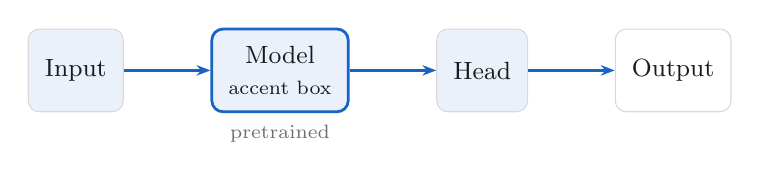
\begin{tikzpicture}[node distance=6mm and 11mm]
    \node[flowbox] (in) {Input};
    \node[flowaccent, right=of in] (enc) {Model\\\scriptsize accent box};
    \node[flowbox, right=of enc] (dec) {Head};
    \node[flowboxw, right=of dec] (out) {Output};
    \draw[flowarr] (in) -- (enc); \draw[flowarr] (enc) -- (dec); \draw[flowarr] (dec) -- (out);
    \node[flowlbl, below=2pt of enc] {pretrained};
  \end{tikzpicture}
  \end{center}
  \vfill
  \centering\sub{Styles \texttt{flowbox}, \texttt{flowboxw}, \texttt{flowaccent}, \texttt{flowarr} and \texttt{flowlbl} ship in \texttt{theme/\_shared.tex}.}
\end{frame}

% =====================================================================
\section{Results}

\begin{frame}{Headline metrics}
  \vfill
  \metricrow{96.5}{accuracy (\%)}{2.4$\times$}{faster}{0}{labels needed}
  \vfill
  \centering\sub{\texttt{\textbackslash metricrow\{\}\{\}...} renders three big accent numbers with captions.}
\end{frame}

\begin{frame}{A results table}
  \centering {\small Benchmark — lower cost is better}\\[0.5em]
  \begin{tabular}{l c c}
    \toprule
    \textbf{Method} & \textbf{Score} & \textbf{Cost} \\
    \midrule
    Baseline      & 81.2 & high \\
    Prior work    & 88.0 & medium \\
    \textbf{This theme} & \acc{\textbf{96.5}} & \acc{low} \\
    \bottomrule
  \end{tabular}
  \vfill
  \sub{\texttt{booktabs} tables look crisp; highlight a row with \texttt{\textbackslash acc\{\}}.}
\end{frame}

% =====================================================================
\section{Closing}

\begin{frame}{Takeaways}
  \begin{enumerate}
    \item A \acc{modern}, minimal Beamer look with almost no configuration.
    \item Everything reusable lives in \texttt{theme/} — restyle in one place.
    \item Build with \acc{Tectonic}: \texttt{./build.sh} $\to$ \texttt{slides.pdf}.
  \end{enumerate}
  \vfill
  \centering\sub{Fork it, change the title, and present.}
\end{frame}

% ---------- closing (no nav / footer) ----------
{\setbeamertemplate{headline}{}\setbeamertemplate{footline}{}
\begin{frame}[plain]
  \centering\vfill
  {\fontsize{36}{40}\selectfont\color{AppleInk}Thank you.}
  \vfill
\end{frame}}

\end{document}
